\chapter{Especificación de Requisitos} \label{requisitos}

\section{Propósito}
En este capítulo se definirán las distintas características, funcionalidades y restricciones que debe cumplir la aplicación que se va a desarrollar. Se redactará un conjunto de requisitos esenciales que guiarán el proceso de creación del sistema. Además, se describirán los requisitos de las interfaces visuales, estableciendo un patrón a seguir durante el desarrollo de la aplicación.

\section{Alcance}
El sistema tiene como objetivo proporcionar a los usuarios una solución eficaz para la búsqueda y gestión de viviendas compartidas, alineada con los principios del \textit{co-housing}. Este proyecto abordará las siguientes tareas principales:

\begin{itemize}
    \item Registro y gestión de usuarios.
    \item Registro y gestión de comunidades.
    \item Recomendación de viviendas por afinidad.
    \item Gestión de tareas y actividades.
\end{itemize}

Los datos serán almacenados en bases de datos, y se hará especial énfasis en la escalabilidad y robustez de la aplicación, con el objetivo de garantizar un rendimiento escalable y efectivo.


\section{Definiciones, siglas y abreviaturas}
\begin{itemize}
    \item \textbf{Usuario Buscador:} Persona que se da de alta en la plataforma con el rol de \textit{Buscador}. Su objetivo es buscar comunidades y unirse a ellas. Puede enviar solicitudes e interactuar con el gestor de tareas.
    \item \textbf{Usuario Ofertante:} Persona que registra una comunidad en la plataforma, introduciendo datos específicos como fotos, metros cuadrados, número de habitaciones, entre otros. Se le ofrecerá funcionalidad para administrar la comunidad, definiendo sus criterios de afinidad y gestionando las solicitudes de unión, aceptándolas o rechazándolas.
    \item \textbf{Comunidad:} Concepto que hace referencia a la vivienda compartida entre varios integrantes. Esta podrá ser gestionada a través de actividades y tareas que se propondrán y deberán ser realizadas por los integrantes de la comunidad.
    \item \textbf{ShareSpace:} Nombre por el que será identificado el proyecto, por tanto a partir de ahora su uso referencia a la aplicación.
\end{itemize}



\section{Perspectiva del producto}
Este sistema tiene como objetivo ofrecer una solución eficiente que adapte las distintas necesidades de los usuarios.
A medida que la aplicación vaya creciendo se podría integrar nueva funcionalidad que aporte valor añadido a la experiencia del usuario.
De forma inicial la aplicación se construirá en torno a distintos servicios que encapsularán parte de la lógica de negocio. Como se puede ver en la imagen \ref{fig:diagrama-componentes} estos componentes se comunicarán con la interfaz gráfica, facilitando la experiencia de usuario de manera sencilla y accesible.
\newpage
\begin{figure}[H]
    \centering
    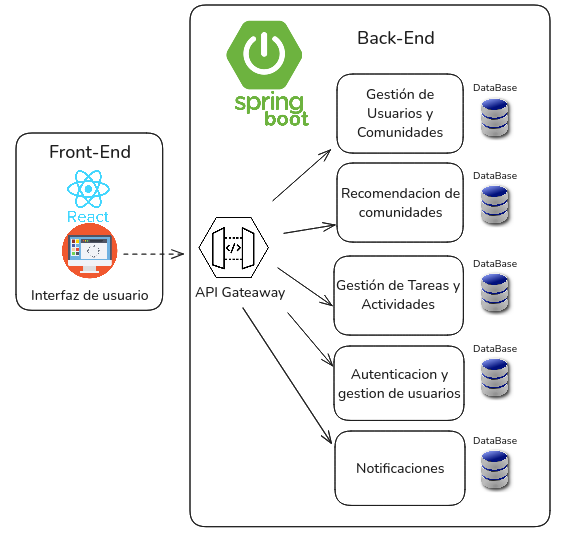
\includegraphics[width=0.8\textwidth]{fotos/diagrama-componentes.png}
    \caption{Diagrama interacción entre componentes\textbf{}.}
    \label{fig:diagrama-componentes}
\end{figure}
\section{Restricciones}
Las restricciones principales de la aplicación para que la experiencia sea la adecuada tanto en móvil como en ordenador serán las siguientes:

\begin{itemize}

    \item \textbf{Hardware:}
    \begin{itemize}
        \item Se recomienda tener al menos 8 GB de RAM para un rendimiento óptimo cuando se usen múltiples pestañas o aplicaciones al mismo tiempo.
    \end{itemize}

   \item \textbf{Navegadores Web:}
    \begin{itemize}
        \item Google Chrome versión 90 o superior.
        \item Mozilla Firefox versión 80 o superior.
        \item Safari 14.0 o superior.
        \item Microsoft Edge versión 90 o superior.
    \end{itemize}
    \item \textbf{Sistemas Operativos Compatibles:}
    \begin{itemize}
        \item \textbf{Windows:} Windows 10 o superior.
        \item \textbf{macOS:} macOS 10.15 o superior.
        \item \textbf{Linux:} Cualquier distribución moderna de Linux, como Ubuntu 20.04 o superior.
    \end{itemize}
\end{itemize}
\section{Funciones del producto}
El sistema contará con una serie de funcionalidades clave para garantizar su cumplimiento del objetivo establecido. A continuación, se detallan las principales funciones que ofrecerá la plataforma:
\begin{itemize}
    \item \textbf{Registro de usuarios y comunidades:} El sistema permitirá registrar tanto a usuarios como a comunidades, gestionando sus respectivos datos. Los usuarios podrán crear su perfil y las comunidades podrán ser configuradas con detalles como ubicación, número de habitaciones, y características específicas.
    \item \textbf{Búsqueda de comunidad:} La plataforma ofrecerá recomendaciones de comunidades basadas en afinidad y preferencias del usuario. Además, permitirá enviar solicitudes de unión a los propietarios de las comunidades, estableciendo una comunicación directa entre ambos para facilitar el proceso de integración.
    \item \textbf{Gestión de tareas:} Los usuarios podrán registrar nuevas tareas, asignarlas a la  comunidad y consultar el estado de las que tienen que realizar. Las tareas estarán integradas en un calendario compartido, asegurando que todos los miembros estén al tanto de las actividades pendientes y los plazos de realización.
    \item \textbf{Gestión de eventos y actividades:} Se podrán crear y gestionar eventos dentro de la comunidad, desde reuniones hasta actividades sociales, fomentando la convivencia.
\end{itemize}

\section{Redacción de requisitos}
Los requisitos van a describir de forma clara y directa las características que el sistema debe proporcionar.  
Vamos a encontrar tres secciones generales:

\begin{itemize}
    \item \textbf{Requisitos funcionales:} Definen las funciones que la aplicación debe ser capaz de realizar.
    \item \textbf{Requisitos no funcionales:} Evaluaran cómo debe comportarse el sistema, dentro de ellos se definiran los requisitos de seguridad.
    \item \textbf{Requisitos de interfaces:} Especificarán los criterios a seguir en el apartado visual, el análisis de las interfaces de usuarios se va a realizar a partir de dos bocetos.
\end{itemize}

Los requisitos funcionales se agruparán en función de grandes bloques de funcionalidad.

\section{Requisitos funcionales}

\subsection{Bloque Gestión de Usuarios y Autenticación}

\begin{itemize}
    \item \textbf{RF-01: Registro de Usuarios}  
    Los usuarios podrán registrarse como buscadores u ofertantes en la aplicación mediante un formulario que recopile información básica. Los campos mínimos requeridos son:
    \begin{itemize}
        \item Nombre
        \item Correo Electrónico
        \item Contraseña
        \item Localización
        \item Afinidad
    \end{itemize}
    
    \item \textbf{RF-02: Inicio de Sesión}  
    Los usuarios podrán iniciar sesión introduciendo su correo electrónico y contraseña previamente registrados.  
    En caso de error en los datos, el sistema notificará al usuario con un mensaje adecuado.
    
    \item \textbf{RF-03: Gestión de Perfiles}  
    Los usuarios deberán poder visualizar y modificar sus datos personales, como la localización y preferencias de afinidad.

    \item \textbf{RF-04: Eliminación de Usuario}
    Los usuarios podrán borrar su cuenta del sistema, eliminando toda información asociada con ellos.
\end{itemize}

\subsection{Bloque Gestión de Comunidades}

\begin{itemize}
    \item \textbf{RF-05: Creación de Comunidades}  
    Los ofertantes podrán crear nuevas comunidad mediante un formulario que incluirá:
    \begin{itemize}
        \item Imágenes representativas
        \item Descripción detallada de la comunidad
        \item Criterios de afinidad para los miembros
        \item Número de integrantes deseado
    \end{itemize}
    
    \item \textbf{RF-06: Unión a Comunidades}  
    Los propietarios deben recibir una notificación cuando un usuario solicite unirse a una comunidad pudiendo ver su información y aceptarlo o rechazarlo.

    \item \textbf{RF-07: Petición de Unión}  
    Los usuarios podrán solicitar unirse a una comunidad concreta mediante un proceso de petición sencilla.

    \item \textbf{RF-08: Notificación de respuesta a Unión}  
    Los usuarios serán notificados con la decisión del propietario de la comunidad a la que han pedido unirse.

    \item \textbf{RF-09: Eliminación de Comunidad}  
    Los propietarios deben poder eliminar la comunidad que han registrado previamente, eliminando toda la información contenida en el sistema.

    \item \textbf{RF-10: Gestión de Comunidad}  
    Los usuarios ofertantes podrán modificar los datos del perfil de la comunidad.


    
\end{itemize}

\subsection{Bloque Gestión de Tareas}

\begin{itemize}
    \item \textbf{RF-11: Creación de Tareas/Eventos}  
    Los usuarios podrán crear tareas/eventos comunitarios mediante un formulario sencillo donde introducirán mínimo: el nombre, una descripción breve y la frecuencia con la que se deberá realizar.
    
    \item \textbf{RF-12: Gestión del Calendario}  
    El sistema debe mostrar un calendario personalizado a cada usuario, que incluirá:
    \begin{itemize}
        \item Tareas asignadas
        \item Eventos destacados
    \end{itemize}
    
    \item \textbf{RF-13: Visibilidad de las Tareas}  
    Los usuarios podrán ver la descripción detallada de cada tarea que se les haya asignado, incluyendo fechas de realización y compañeros con los que tienen que colaborar.
    
    \item \textbf{RF-14: Marcar Tareas}  
    Los usuarios deberán poder marcar las tareas como completadas y consultar el estado de las tareas pendientes con su respectiva fecha límite.

    \item \textbf{RF-15: Reparto de Tareas}  
    El sistema distribuirá las tareas semanalmente de manera justa, asignando responsabilidades en un orden secuencial.

    \item \textbf{RF-16: Flexibilidad en la Asignación de Tareas}  
    Los usuarios podrán distribuir de forma libre sus tareas asignadas a lo largo de la semana.
\end{itemize}

\subsection{Bloque Recomendación de Comunidades}

\begin{itemize}
    \item \textbf{RF-17: Recomendación de Comunidades}  
    El sistema recomendará comunidades que coincidan con los criterios tanto de afinidad como de vivienda introducidos por los usuarios.
    
    \item \textbf{RF-18: Guardar Comunidades de Interés}  
    El usuario podrá guardar sus comunidades de interés utilizando un botón de “guardar” o “me gusta”.
    
    \item \textbf{RF-19: Grado de afinidad}  
    El sistema mostrará a los usuarios el grado de afinidad que existe entre una comunidad y ellos con un porcentaje sobre cien.
\end{itemize}

\section{Requisitos No Funcionales}
\begin{itemize}
    \item \textbf{RNF-01: Notificaciones}  
    Las notificaciones deben ser rápidas y entregarse a los usuarios en un período de tiempo corto (entorno a uno o dos segundos).
    
    \item \textbf{RNF-02: Mantenibilidad y Escalabilidad}  
    El sistema debe estar diseñado para ser fácil de mantener, pudiendo escalar a medida que crecen los usuarios y las funcionalidades.
    
    \item \textbf{RNF-03: Alta Disponibilidad}  
    El sistema debe permanecer operativo en todo momento, asegurando que si aparece un fallo en alguna parte del sistema el resto de servicios seguirán operativos.
    
    \item \textbf{RNF-04: Soporte de Carga}  
    El sistema debe soportar un volumen de usuarios considerable de forma simultánea, asegurando que el servicio esté disponible ante un flujo alto de usuarios.

    \item \textbf{RNF-05: Mantenimiento}
    El sistema debe permitir al administrador realizar tareas de mantenimiento sin afectar el servicio a los usuarios
    \item \textbf{RFN-06: Gestión de Usuarios}
    El sistema debe poder permitir al administrador gestionar los usuarios pudiendo activar/desactivar cuentas y modificar roles.
    \item \textbf{RFN-07: Monitoreo}
    El sistema debe alertar al usuario en caso de caídas de servicio que afecten a los usuarios.
\end{itemize}

\subsection{Requisitos de Seguridad}
\begin{itemize}
    \item \textbf{RNF-08: Autorización y autenticación}  
     La aplicación deberá contar con un sistema de autenticación y autorización seguro que garantice el control de los accesos.
    
    \item \textbf{RNF-09: Seguridad en Base de Datos}  
    El sistema debe implementar mecanismos de seguridad que protegan a las bases de datos de accesos no autorizados.
    
    \item \textbf{RNF-10: Protección contra Inyecciones SQL}  
    El sistema debe prevenir ataques de inyección SQL mediante el uso de validaciones adecuadas en los datos de entrada.
    \item \textbf{RNF-11: Protección de datos}
    El sistema debe asegurar el cumplimiento de las normativas vigentes de  \href{https://eur-lex.europa.eu/ES/legal-content/summary/general-data-protection-regulation-gdpr.html}{protección de datos de la Unión Europea}, para garantizar un uso adecuado de los datos personales.
\end{itemize}

\subsection{Requisitos de Interfaces Externas}
Dentro de las interfaces externas distinguimos dos grandes bloques, las APIs y las Interfaces de usuario:

\subsubsection{APIs}
Cada servicio del sistema expondrá sus operaciones a través de una API, lo que permitirá una comunicación eficiente entre los módulos.


\subsubsection{Interfaces de Usuario}

La interfaz de usuario permitirá un uso de la funcionalidad ofrecida por el sistema claro y sencillo.

Cada interfaz va a cumplir una serie de criterios de usabilidad y una estética uniforme. A modo de ejemplo se va a presentar dos bocetos esquematizados para presentar el flujo de diseño a seguir.

\subsubsection*{Página de Bienvenida}
La ''Landing Page'' tiene como objetivo ser la puerta de entrada a la aplicación para el usuario, por lo tanto tiene que ser directa y llamativa para captar su atención.
\newpage
\begin{figure}[H]
    \centering
    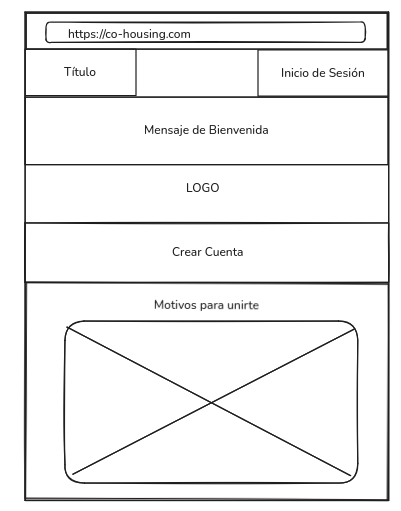
\includegraphics[width=0.8\textwidth]{fotos/home-basico.png}
    \caption{Boceto ''Landing Page''\textbf{}.}
    \label{fig:landing-page}
\end{figure}
\subsubsection*{Descripción:}
La imagen \ref{fig:landing-page} muestra la página a la que accede el usuario mediante el buscador al introducir el nombre de la aplicación, esta tiene como objetivo mostrar una pequeña presentación de la app y permitir la realización de una acción muy concreta, en este caso registrarse o iniciar sesión.

\newpage

\subsubsection*{Página Buscador}
La página del buscador tiene como objetivo poner en contacto a los usuarios con comunidades afines por lo que se debe mostrar la información de manera clara y bien estructurada.

\begin{figure}[H]
    \centering
    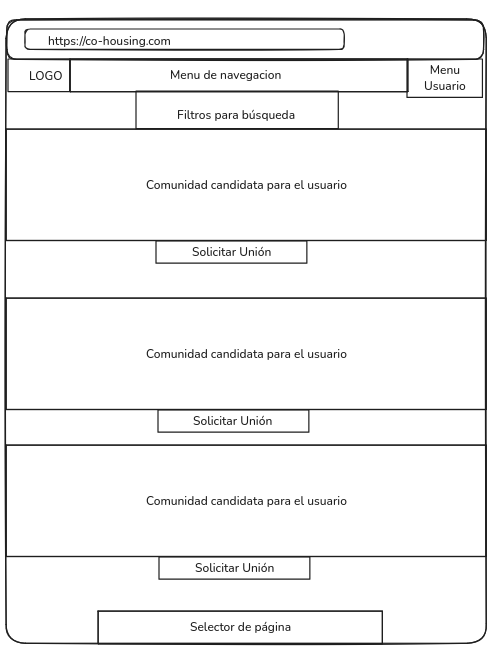
\includegraphics[width=0.8\textwidth]{fotos/buscador-basico.png}
    \caption{Boceto Página Buscador\textbf{}.}
    \label{fig:buscador-page}
\end{figure}
\subsubsection*{Descripción}
La imagen \ref{fig:buscador-page}  muestra la página que visualizará el usuario cuando accede a la sección ''Buscador'' de la aplicación,en ella aparecen las distintas comunidades sugeridas y un botón para solicitar la unión, además cuenta con un menú de navegación y un menú para el usuario.


